\documentclass[twocolumn,11pt]{article}

\usepackage[utf8]{inputenc}
\usepackage{lipsum}                     % Dummytext
\usepackage{hyperref}
\usepackage{xargs}                      % Use more than one optional parameter in a new commands
\usepackage[pdftex,dvipsnames]{xcolor}  % Coloured text etc.
\usepackage{graphicx}
\usepackage{verbatim}
\usepackage{float}
\usepackage{tikz-qtree}
\usepackage{tikz}
\usepackage[linguistics]{forest}

\usepackage{amssymb}
\usepackage{amsmath}
\newcommand*{\QEDA}{\hfill\ensuremath{\blacksquare}}% filled box
\newcommand*{\QEDB}{\hfill\ensuremath{\square}}% unfilled box

% dem nice tables
\usepackage[hmargin=2cm,top=4cm,headheight=65pt,footskip=65pt]{geometry}
\usepackage{fmtcount} % for \ordinalnum
\usepackage{array,multirow}
\usepackage{tabularx}
\usepackage{lastpage}


% add a special collumn type
\newcolumntype{C}[1]{>{\centering\arraybackslash}m{#1}}


%header/footer stuff
\usepackage{fancyhdr}
\pagestyle{fancy}

%note that if you do not do these blank ones, the package defaults to something
%you may not want in your header or footer
\lhead{CMPS 278}
\chead{RocksBench}
\rhead{\today}
\lfoot{Isaak Cherdak}
\cfoot{}
\rfoot{\thepage}

\renewcommand{\headrulewidth}{0pt}
\renewcommand{\footrulewidth}{0pt}

\hypersetup{
    colorlinks=true,
    linkcolor=blue,
    filecolor=magenta,
    urlcolor=cyan,
}

\usepackage[english]{babel}
\emergencystretch=1pt
\usepackage[justification=centering]{caption}
\graphicspath{{Pictures/} }

\usepackage[colorinlistoftodos,prependcaption,textsize=tiny]{todonotes}
\newcommandx{\unsure}[2][1=]{\todo[linecolor=red,backgroundcolor=red!25,bordercolor=red,#1]{#2}}
\newcommandx{\change}[2][1=]{\todo[linecolor=blue,backgroundcolor=blue!25,bordercolor=blue,#1]{#2}}
\newcommandx{\info}[2][1=]{\todo[linecolor=OliveGreen,backgroundcolor=OliveGreen!25,bordercolor=OliveGreen,#1]{#2}}
\newcommandx{\improvement}[2][1=]{\todo[linecolor=Plum,backgroundcolor=Plum!25,bordercolor=Plum,#1]{#2}}
\newcommandx{\thiswillnotshow}[2][1=]{\todo[disable,#1]{#2}}

%\usepackage{setspace}
%\doublespacing

\title{RocksBench\\CMPS 278}
\author{Isaak Cherdak}
%\date{} %blank date

\begin{document}

\maketitle

\pagebreak

\section*{Notation}

\begin{center}
  \begin{tabular}{ | l | l | }
    \hline
    Abbreviation & Expanded Phrase or meaning\\ \hline \hline
    DBMS & Database Management System\\ \hline
    SLA & Service Level Agreement\\ \hline
  \end{tabular}
\end{center}

\section{Introduction}
\label{sec:overview}

RocksDB is a popular DBMS used in applications ranging from storing data for
Netflix to being a component of other database services like MongoDB. This is
very impressive as RocksDB was only designed specifically for Facebook's needs:
to lessen the bottleneck of storage space. The general philosophy behind RocksDB
is that as long as the SLA is met, all optimizations should be focused on
decreasing storage space. However, since the best DBMS depends on the use
case\cite{278:lecture}, it is not completely clear as to what situations
would best make use of RocksDB. I present RocksBench, a simple benchmark that
aims to give better insight into the applications where RocksDB would be
especially effective and those where another system may be a better fit.

RocksBench uses various combinations of calls to RocksDB functions. However, it
allows the user to tune parameters to test in as large or small scale as they
would like. RocksBench provides results in csv files. Furthermore, there are a
number of scripts provided to analyze the results as well as plot graphs. The
analysis is done using ascar-pilot\cite{li:pilot}. The graphs are generated via
python's matplotlib library.

\section{Background}
\label{sec:background}

\subsection{My Personal Experience}
\label{subsec:personal_experience}

I have experience setting up Benchmarks in C/C++ for various data structures.
Specifically, I have been able to send multiple experiment trials to a file and
have used pilot, to generate analytics for the results (such as standard
deviation, average, etc). I have also been able to graph these results using
matplotlib. I applied this experience to design an even more dynamic process of
running experiments for RocksDB.

I previously did experiments on four different data structures: Singly Linked
List, Vector, B-Tree, and LSM-Tree. The first three were written by myself in a
consistent manner and the LSM-Tree was adapted based off one created by a
Harvard PhD student. The benchmark was at best able to run 40000 inserts and
40000 get calls with 100 trials in approximately 30 seconds. The order of
inserts and get calls wasn't the same but the way they were run differed
depending on the data structure. The hardware setup was the home PC as described
in \ref{subsec:test_hw} as well as my laptop which had comparable results. Test
results included aggregate runtime of all inserts, aggregate runtime of all
calls to get, and total in-memory size at the end of all insertions. It should
be noted that I was able to run these experiments without having any issues with
memory / storage usage (runtime was main bottleneck) when using an 800 MB NVRAM
pool. Valgrind reported approximately 25 GB of dynamic memory allocating/freeing
over the course of all trials/experiments in the case of 40000 inserts/100
trials.

\subsection{Ascar-Pilot}

Pilot\cite{li:pilot} is an analysis tool created by Yan Li in coordination with
the SSRC. There are three forms: a command line tool for analyzing spreadsheets,
a command line tool for timing a shell command, and a library which can be used
in C++ to time functions. I went with the first system since I was perfectly
fine generating timing data on my own. Pilot was hence used to provide averages
over multiple trials for each type of test as well as variance which was used to
generate error bars for graphs.

\subsection{LSM Trees}

Over the course of the development and deployment of RocksDB, Facebook
determined that the most useful properties of the LSM tree were decreased write
and space amplification. Before this discovery, LSM trees were less popular and
their most major benefit was thought to be decreased random writes to storage.

\subsection{RocksDB}

The RocksDB paper gave a lot of insight into how their system was implemented
and how it worked in practice, even though it didn't provide many particularly
novel ideas.

A major concern I had with the RocksDB paper was the evaluation section. It's
difficult to fairly compare RocksDB with another system since RocksDB only
intends to meet SLA: any differences in performance between other systems are
kind of irrelevant in this regard. The only metric that mattered was storage
size which wasn't any better than InnoDB (with zlib compression) and TokuDB
(with no compression). As such, the message appears to be that RocksDB maintains
reasonable storage optimization while also giving reasonable performance.

\section{RocksBench}

\subsection{Overview}

This Benchmark was designed in C++ and provides command line arguments to let
users customize options for the tests.

different tests with varying ratios of operations (put/get/update/delete). A
single experiment is defined as a single group of operations that is run with at
least 100 trials. The purpose of doing multiple trials is to ensure accuracy of
results.

\subsection{Characterization of tests}
\label{subsec:characterization_tests}

\begin{table}[h!]
  \begin{tabular}{ |c|c|c|c| }
    \hline
    Test Name & R:W:D Ratio & Hit Rate & Data \\
    \hline \hline
    seq\_hit\_read & 1000:10:5 & High & Sequential \\ \hline
    seq\_hit\_write & 10:1000:5 & High & Sequential \\ \hline
    seq\_hit\_delete & 100:10:50 & High & Sequential \\ \hline
    seq\_miss\_read & 1000:10:5 & Low & Sequential \\ \hline
    seq\_miss\_write & 10:1000:5 & Low & Sequential \\ \hline
    seq\_miss\_delete & 100:10:50 & Low & Sequential \\ \hline
    rnd\_hit\_read & 1000:10:5 & High & Random \\ \hline
    rnd\_hit\_write & 10:1000:5 & High & Random \\ \hline
    rnd\_hit\_delete & 100:10:50 & High & Random \\ \hline
    rnd\_miss\_read & 1000:10:5 & Low & Random \\ \hline
    rnd\_miss\_write & 10:1000:5 & Low & Random \\ \hline
    rnd\_miss\_delete & 100:10:50 & Low & Random \\ \hline
  \end{tabular}
  \caption{The twelve different types of tests}
  \label{tab:types_of_tests}
\end{table}

There are twelve different kinds of tests as described in table
\ref{tab:types_of_tests}. Each test strives to show the results of using a
different kind of input set. In practice there is also a level at which database
systems administrators can predict the kind of input they are primarily getting
and optimize for that case. These tests could give some insight and help someone
make a decision about whether RocksDB is right for them.

The limit on the number of operations / memory usage is dependent on that which
is described in \ref{subsec:max_threshold}.

\subsection{Implementation}

RocksBench was designed very carefully in the interest of modularity as well as
to prevent unnecessary operations as the use of the RocksDB functions already
slows the benchmark significantly. It is also relatively scalable: being able to
perform tests with very large base sizes but the largest current tested size is
around 65000.

\begin{table}[h!]
  \begin{tabular}{ |c|c|c|c| }
    \hline
    Option & Description & input type \\
    \hline \hline
    n & lets you specify a prefix for your results folder & string \\ \hline
    b & beginning size & int \\ \hline
    s & end size & int \\ \hline
    m & multiply amount for test size each iteration & float \\ \hline
    t & number of trials & int \\ \hline
    d & debug & None \\ \hline
  \end{tabular}
  \caption{A list of all the options available in RocksBench}
  \label{tab:RocksBench_options}
\end{table}

The Main system allows a user to choose some options. These are listed in table
\ref{tab:RocksBench_options}. Together with these options you can perform tests
according to your needs. RocksBench will run all twelve of the tests described
in section \ref{subsec:characterization_tests} for all sizes starting at the
beginning value, multiplying by the multiplier each time, and going until the
value is bigger than the end size. The folder will be <custom\_name>\_results
where <custom\_name> is "default" by default. The main system will receive a
vector from each trial and create the first line of the file such that it is the
header and all the following lines will only contain data from each trial. The
files are organized in a hierarchy of
custom\_result/test\_type/test\_type\_size.csv. The number of trials can also be
changed to reflect how many times a test should be retried for additional
accuracy.

\subsection{Challenges}

\subsubsection{Benchmark Design}

Designing the benchmark took a large amount of time and consideration because at
any given point the things that I would like to test may change. If the system
was badly written, there would be a large amount of time spent on rewriting
large portions of the system every time a change occurred.

\subsubsection{Utilization of RocksDB library}

The RocksDB library via the github repo didn't have the best example setup so
some time was spent on coming up with a more generalist configuration.
Originally, RocksDB intended for people to use their examples which were
completely hard-coded to make use of the parent directory. I remade their
examples and Makefiles so that compilation was based off the actual install
directory. This was very good for me because by the time I wanted to make use of
the library, I already knew exactly how to correctly link it to the install
locations and make use of their custom configuration file. The other major
challenge was the sheer number of ways that you can do a single put/get/delete
which is why a lot of the tests I use have very simple functionality.

\subsubsection{Test Coverage}

Determining the tests to run was very difficult both due to initial concerns and
those that turned up over the course of the project. Initially, I was aware that
there would be a large number of parameters and as a result, it would be
impossible to make a completely comprehensive test. This led me to choose to
leave options as defaults, which may be something that plenty of users would do
for the same reason. I also initially planned to use varying ratios of
\textit{put}, \textit{get}, \textit{update}, and \textit{delete} calls. However,
as the project progressed I realized that the tests that involved random number
generation resulted in \textit{update} calls during what was supposed to be a
\textit{put} test. As a result, I decided to remove \textit{update} tests from
the variables.

\section{Evaluation}

A lot of graphs were generated due to the ease of use of RocksBench.
Specifically, there were 72 graphs at the end of my experiments. This is because
there is a graph for every operation (put, get, delete) for every type of test
(for which there are 12) and for both computers (my home and lab computer).
Thus, not all graphs are displayed here but they can be viewed here: \href{}{}.
In addition, error bars are implemented but apparently 10 trials was sufficient
to make most data points not even display the error bars.

\subsection{Test Hardware}
\label{subsec:test_hw}

I will be running these tests on a virtual machine on my home desktop as well as
on a direct boot of Linux on my lab machine. My home desktop has a AMD Ryzen R7
1700 CPU, 32 GB 3000MHz DDR4 RAM, and a 500 GB primary storage SSD. The virtual
machine will be using 8 CPU cores, 16 GB RAM, and 50 GB of my SSD. As for my lab
PC, it has an Intel core i5-3550 CPU, 16 GB 1866MHz DDR3 RAM, a 500 GB SSD, ~250
GB of which are being used for the Linux.

\subsection{Maximum Threshold}
\label{subsec:max_threshold}

The range of tests were as large as possible. Experiments were run from 1 to
32768 base size. The next size up would actually be stuck on the first trial of
seq\_miss\_read which makes sense because this test overturned the general rule of
put(), or write, being the fastest.

\subsection{Home PC}

\begin{figure}[h]
  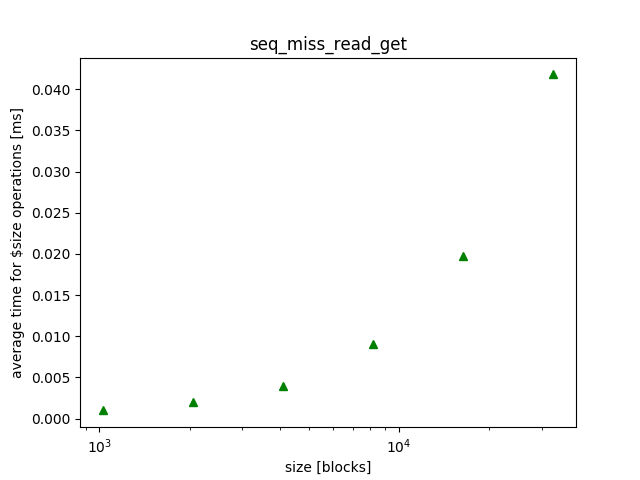
\includegraphics[width=\linewidth]{Pictures/HOMEPC/seq_miss_read_complete_get.png}
  \label{fig:seq_miss_read_get}
\end{figure}[h]
\begin{figure}[h]
  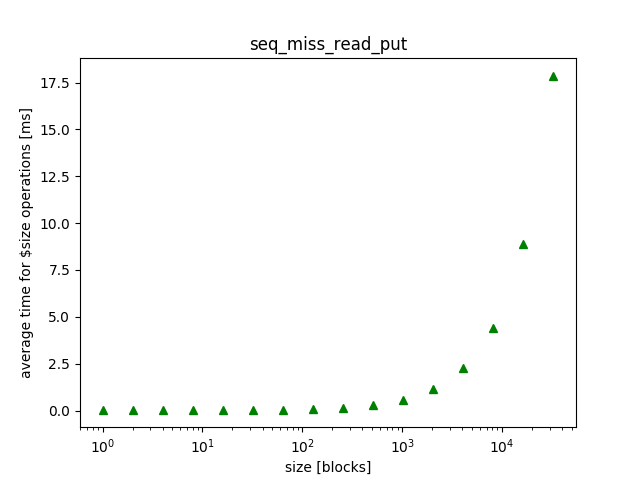
\includegraphics[width=\linewidth]{Pictures/HOMEPC/seq_miss_read_complete_put.png}
  \label{fig:seq_miss_read_put}
\end{figure}[h]

This computer performed much better, likely because of its more modern hardware.
Interestingly enough, it didn't seem to make full use of resources. For any
given test put() was the fastest except for one case: seq\_miss\_get where get()
was multiple orders of magnitude slower. This can

\subsection{Lab PC}

This computer was making heavy use of resources, but even so it was
unsurprisingly slower.

\subsection{Result Insights}
\label{subsec:res_insights}

I observed some interesting results over the course of the variety of tests
performed. Surprisingly, get is still very fast in many situations: contrary to
what one would expect from a LSM tree. However, delete was perhaps the biggest
hit to latency as it would often take very long times for few deletes relative
to reads and writes

Some work could potentially go into figuring out the most optimal hardware. It
was noted that when running tests on the lab computer, one core was often at
100\% while others were down to around 20-30\% utilization. Perhaps this is an
issue only in older processors but my home computer is actually experiencing the
opposite effect. One might expect my home computer to be much faster than the
lab computer given that the former runs at around 10\% CPU usage. However, even
though it is a little faster, it doesn't seem to be making good use of hardware.
Another factor that may cause this is the virtual machine. However, in the past
I have seen disk and memory usage go up to 100\% due to processes in a virtual
machine and currently RocksBench has a negligible affect on both of these
resources.

\section{Future Work}
\label{sec:future_work}

\subsection{RocksDB using NVRAM}

Many additional optimizations are available to systems that have NVRAM. The most
interesting ones appear to be WBL and the ability to not always have to flush
data from memory to storage. Some interesting results could be achieved if a
variety of ratios of RAM vs NVRAM were used to benchmark a NVRAM functioning
RocksDB.

RocksDB can be modified to use NVRAM. Furthermore, even with difficulty to
attain physical NVRAM, it is possible to emulate it using Intel's step-by-step
guide\footnote{
  \href{https://software.intel.com/en-us/articles/how-to-emulate-persistent-memory-on-an-intel-architecture-server/}
  {Intel NVRAM Emulation Guide}}.
To make use of the NVRAM, regardless of whether it's emulated: the Intel PMDK
library can be used (formerly known as NVML). A perfectly sufficient module
provided by PMDK called libpmemobj
\footnote{\href{http://pmem.io/pmdk/libpmemobj/}
{PMDK libpmemobj documentation}} allows a user to make use of syntax reminiscent
of malloc and free while also providing a persist call.

\subsection{Expanding coverage of the testbench}

RocksBench currently only makes use of very simple calls to RocksDB using the
default options. On one hand this isn't so bad since many users may choose to do
the same since Facebook has chosen default options quite reasonably and because
of the overwhelming variety of methods to make use of the Database. However,
transactions would likely also be used as well as methods common with the
backwards compatible LevelDB API. Luckily, the structure of the database is very
modular and would make such additions relatively painless once they are
independently planned and designed.

\subsection{Research into optimal hardware setup}

As mentioned before like in section \ref{subsec:res_insights}, there may be more
nuance than has ever been considered regarding the kinds of hardware that makes
the database system operate more efficiently.

\subsection{Level A}

Characterization of major use cases of RocksDB and discussion of optimizations
that would further increase the range of use cases. This involves running
various benchmarks and analysis of the results as described in
\ref{subsec:characterization_tests}.

\subsection{Level B}

This involves the work proposed in Level A as well as tests on an optimized
version of RocksDB. This optimization would likely be a modified version of
RocksDB so that it runs on NVRAM as described in \ref{subsec:opt_rocksdb}.

\subsection{Level C}

This would involve Level A, B, and the application of Levels A and B to LevelDB.
Finally, a comparison of the use cases between the two systems which will simply
include the Level A analysis of both systems. This will also include a
discussion of the cost-benefit of some of the features added to RocksDB which
LevelDB did not have.


\bibliographystyle{abbrv}
\bibliography{rocksbench,bib/csrg}

\end{document}
